\chapter{直线和平面}
\section{空间图形}
在初中几何课中,我们讨论的几何图形和几何问题,主
要局限在一个平面上。然而,我们生活着的现实世界却是具
有长、宽、高的所谓“三维空间”。而平面只是我们生活空
间的某个断面。我们日常所见的形体,如桌椅、房屋、球、
漏斗等等,它们并不局限在一个平面上,都是立体的。为了
精确地认识这些实际存在的形体,以便为我们的生产和生活
服务,我们必须学习有关空间图形的知识。

我们知道平面图形是同一平面上的点的集合,而\textbf{空间图
形却是不全在同一平面上的点的集合}。例如正方体、三棱
锥、圆柱、球等都是空间图形。空间图形也叫立体图形。我
们将在平面几何知识的基础上,来研究空间图形的性质、画
法以及有关的计算和应用。

\begin{figure}[htp]
    \centering
%\includegraphics[scale=.4]{fig/1-1.png}
    \caption{}
\end{figure}

空间图形是在平面上(纸上)画出来的表示立体的图。
如在图1.1中,各图都表示出了某种立体。这种图形叫直
观图。除了用直观图表示立体以外,还有其他表示立体的方
法,如展开图和投影图等等。下面我们作些简要的介绍。

\subsection{直观图}
\subsubsection{水平放置的平面图形的画法}
当我们把一个正方形和圆放置在水平位置观察时,我们
的视觉会产生一些变化,总觉得它们像平行四边形和椭圆。
它们会变成怎样的平行四边形和椭圆呢?由于观察的角度不
同,会有不同的形状,这就涉及到了水平平面图形的画法问
题,下面就是较常用的两种画法。

第一种画法

\begin{example}
    画正方形的直观图。
\end{example}

\begin{figure}[htp]
    \centering
    \begin{tikzpicture}[>=latex,scale=1.5]
     \begin{scope}
\draw[<->](1.5,0)node[right]{$X$}--(0,0)--(0,1.5)node[right]{$Y$};
\draw(0,0)node[below]{$A$}--(1,0)node[below]{$B$}--(1,1)node[right]{$C$}--(0,1)node[left]{$D$};
\node at (.8,-.5,0){$(1)$};
\end{scope}   
\begin{scope}[xshift=3cm, x={(0:1cm)},y={(45:.5cm)},z={(90:1cm)}]
    \draw[<->](2,0,0)node[right]{$X'$}--(0,0,0)--(0,2,0)node[right]{$Y'$};
    \draw(0,0,0)node[below]{$A'$}--(1,0,0)node[below]{$B'$}--(1,1,0)node[right]{$C'$}--(0,1,0)node[left]{$D'$};
    \node at (1.5,-1.414,0){$(2)$};
    \end{scope}      
    \end{tikzpicture}
    \caption{}
\end{figure}

\textbf{画法}
\begin{enumerate}
    \item 在正方形$ABCD$上,分别取$AB$、$AD$为$X$轴
和$Y$轴,它们互相垂直于$A$点。

画对应的$X'$轴和$Y'$轴,使$\angle X'A'Y'=45^{\circ}$.
\item 在$X'$轴上截取$A'B'=AB$, 在$Y'$轴上截取
$A'D'=\frac{1}{2}AD$

\item 以$A'B'$、$A'D'$为邻边画平行四边形
$A'B'C'D'$就是正方形$ABCD$的直观图。(图1.2)。
\end{enumerate}

\begin{example}
    画正五边形的直观图。
\end{example}


\begin{figure}[htp]
    \centering
    \begin{tikzpicture}[>=latex,scale=1.2]
     \begin{scope}
\draw[<-](0,4)node[right]{$Y$}--(0,-.5); 
\draw[->](-2,0)--(2,0)node[right]{$X$};
\draw(-1,0)node[below]{$A$}--(1,0)node[below]{$B$}--(1.62,1.9)node[right]{$C$}--(0,3.08)node[right]{$D$}--(-1.62,1.9)node[left]{$E$}--(-1,0);
\draw[dashed](-1.62,1.9)--(-1.62,0)node[below]{$E_1$};
\draw[dashed](1.62,1.9)--(1.62,0)node[below]{$C_1$};
\node at (.25,-.25){$O$};
\node at (0,-1){$(1)$};
\end{scope}   
\begin{scope}[xshift=5cm, x={(0:1cm)},y={(45:.5cm)},z={(90:1cm)}]
    \draw[<-](0,6)node[right]{$Y'$}--(0,-1); 
    \draw[->](-2,0)--(3,0)node[right]{$X'$};
    \draw(-1,0)node[below]{$A'$}--(1,0)node[below]{$B'$}--(1.62,1.9)node[right]{$C'$}--(0,3.08)node[right]{$D'$}--(-1.62,1.9)node[left]{$E'$}--(-1,0);
    \draw[dashed](-1.62,1.9)--(-1.62,0)node[below]{$E'_1$};
    \draw[dashed](1.62,1.9)--(1.62,0)node[below]{$C'_1$};
    \node at (.25,-.5){$O'$};
    \node at (1,-2.828,0){$(2)$};
    \end{scope}      
    \end{tikzpicture}
    \caption{}
\end{figure}

\textbf{画法}
\begin{enumerate}
    \item 取正五边形$ABCDE$的$AB$所在直线为$X$轴,
    取$AB$的中垂线为$Y$轴($Y$轴必过$D$点),两轴交于$O$点.
    (图1.3(1))

    画对应的$X'$轴,$Y'$轴,使$\angle X'O'Y'=45^{\circ}$
    \item 作$CC_1\bot X$轴于$C_1$, 作$EE_1\bot X$轴于$E_1$, 在
    $X'$轴上取$A'B'=AB$, 且使$O'$为$A'B'$中点,并在$X'$轴
    上分别取$C'_1$点和$E'_1$点,使$O'C'_1=OC_1$, $O'E'_1=OE_1$.
    \item 在$Y'$轴上截取$O'D'=\frac{1}{2}OD$, 并引$E'_1E'\parallel
    O'Y'$, 且使$E'_1E=\frac{1}{2}E_1E$, 引$C_1'C'\parallel O'Y'$, 且使
    $C'_1C'=\frac{1}{2}C_1C$.
    \item 连结$A'E'$、$E'D'$、$D'C'$、$C'B'$, 则五边
    形$A'B'C'D'E'$就是正五边形$ABCDE$的直观图。(图
    1.3(2))
\end{enumerate}

通过上面例题,我们可以得出这种画法的规则如下:
\begin{enumerate}
\item 在图形上取互相垂直的$X$轴、$Y$轴,并画出与之
对应的$X'$轴,$Y'$轴,使$\angle X'O'Y'=45^{\circ}$(或$135^{\circ}$), $X'$
轴和$Y'$轴所确定的平面表示水平平面。
\item 图形中平行于$X$轴或$Y$轴的线段(包括在轴上的
线段)分别画成平行于$X'$轴和$Y'$轴的线段。
\item 平行于$X$轴的线段,长度不变;平行于$Y$轴的线
段,长度变为原来的一半。
\end{enumerate}

第二种画法

\begin{example}
   画圆的直观图 

   圆的直观图是一个椭圆,常采用如下近似画法:
\begin{enumerate}
    \item 取$\odot O$的一对互相垂直的直径$AB$, $CD$分别为$X$
轴、$Y$轴,并画出对应的$X'$轴、$Y'$轴,使$\angle X'O'Y'=120^{\circ}$.
\item 在$O'X'$上取$O'A'=OA$, 并取$A'$关于$O'$的对称
点$B'$, 然后在$O'Y'$轴上取$O'C'=OC$, 并取$C'$关于$O'$的对
称点$D'$.
\item 过$A'$、$B'$作$O'Y'$的平行线,过$C'$、$D'$作$O'X'$
的平行线,所作四条直线交出一个菱形,设$E$、$F$是菱形关
于$O'$点对称的顶点。
\item 连$ED'$, $FA'$, 交于$G$; 连$EB'$、$FC'$交于$H$.
\item 以$E$为心,以$ED'$为半径,作$\wideparen{D'B'}$, 以$F$为心,
以$FA'$为半径作$\wideparen{A'C'}$, 以$G$为心,以$GA'$为半径作$\wideparen{D'A}$,
以$H$为心,以$HC'$半径作$\wideparen{B'C'}$, 则此四弧连接成一个近似椭
圆.(图1.4(2))
\end{enumerate}

\begin{figure}[htp]
    \centering
    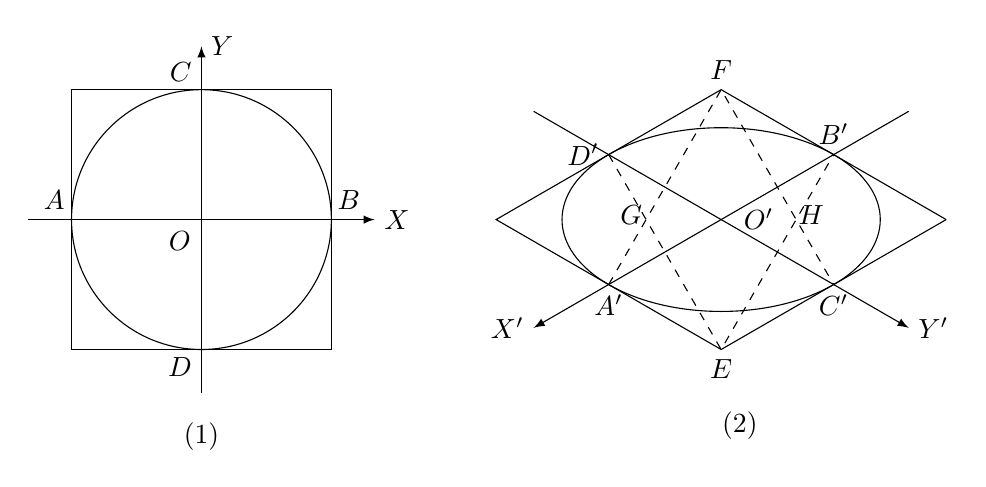
\begin{tikzpicture}[>=latex,scale=1.1]
     \begin{scope}
\draw[<-](0,2)node[right]{$Y$}--(0,-2); 
\draw[->](-2,0)--(2,0)node[right]{$X$};
\draw(-1.5,-1.5)--(-1.5,1.5)--(1.5,1.5)--(1.5,-1.5)--(-1.5,-1.5);
\draw (0,0) circle (1.5);
\node at (-1.7,0)[above]{$A$};
\node at (1.7,0)[above]{$B$};
\node at (0,1.7)[left]{$C$};
\node at (0,-1.7)[left]{$D$};
\node at (-.25,-.25){$O$};
\node at (0,-2.5){$(1)$};
\end{scope}   
\begin{scope}[xshift=6cm, x={(-150:1cm)},y={(150:1cm)}]
    \draw[->](0,2.5)--(0,-2.5)node[right]{$Y'$}; 
    \draw[->](-2.5,0)--(2.5,0)node[left]{$X'$};
    \draw(-1.5,-1.5)--(-1.5,1.5)--(1.5,1.5)--(1.5,-1.5)--(-1.5,-1.5);
    \draw (0,0) circle (1.5);
    \node at (-1.5,0)[above]{$B'$};
    \node  at (1.5,0)[below]{$A'$};
    \node  at (0,1.5) [left]{$D'$};
    \node  at (0,-1.5)[below]{$C'$};
    \node  at (-.25,-.25){$O'$};
    \node  at (.55,.65){$G$};
    \node  at (-.65,-.55){$H$};
    \draw[dashed](0,1.5)--(1.5,-1.5)node[below]{$E$}--(-1.5,0);
    \draw[dashed](1.5,0)--(-1.5,1.5)node[above]{$F$}--(0,-1.5);
    \node at (2.25,-2.5){$(2)$};
    \end{scope}      
    \end{tikzpicture}
    \caption{}
\end{figure}

从上述画法中,我们看出圆的中心$O$, 变成了椭圆的中
心$O'$, 圆的一对互相垂直的直径(如$AB$、$CD$)变成椭圆
的一对直径(如$A'B'$, $C'D'$),它们叫做椭圆的共轭直
径,实际上如果知道了一对椭圆的共轭直径,就可以把椭圆
近似地画出来了。

更省事的办法是用椭圆模板(图1.5)经过椭圆的一对
共轭直径端点来画椭圆。
\begin{figure}[htp]
    \centering
%\includegraphics[scale=.7]{fig/1-5.png}
    \caption{}
\end{figure}

从上例中可以看到:\textbf{第二种画法与第一种画法不同的,只
是$\angle X'O'Y'=120^{\circ}$;并且平行于$Y$轴的线段的长度不变}.

注意:直观图画好以后,要擦去辅助线。
\end{example}

\begin{ex}
\begin{enumerate}
\item 任意画一个三角形,然后用两种方法画出它们的直观图。
\item 任意画一个长方形,然后用两种方法画出它们的直观图。
\item 已知椭圆的一对共轭直径$AA'$、$BB'$, 近似地画出这个
椭圆。
\item 画一个边长为1.5cm的正六边形,然后用两种方法画出
它的直观图。
\end{enumerate}

(注意:以上练习只要求精确而美观地画出图形,不要
求写作法。)
\end{ex}

\subsubsection{空间形体的直观图}
\begin{example}
    画一个长、宽、高分别为3cm, 2cm和1.5cm的长
方体的直观图。
\end{example}

第一种画法:
\begin{enumerate}
    \item 在水平平面上画$X'$轴和$Y'$轴,两轴交于$O'$点,
    且使$\angle X'O'Y'=135^{\circ}$.
    \item 在$O'X'$上取$O'P'=1$cm, 在$O'Y'$上取$O'S'=
    3$cm, 作$S'R'\parallel O'X'$, $P'R'\parallel O'Y'$, 则平行四边形$O'P'R'S'$
    为已知长方体的底面的直观图。
    \item 过$O'$点作$Z'$轴垂直于$Y'$轴,并在$O'Z'$上取$OO'
    =1.5$cm, 过$P'$、$R'$、$S'$分别作$PP'\parallel O'Z'$, $RR' \parallel O'Z'$,
    $SS'\parallel O'Z'$, 并且,$PP'=RR'=SS'=1.5$cm.
    \item 连$OP$、$PR$、$RS$、$SO$, 则$PRSO-P'R'S'O'$
    为已知长方体的直观图。(图1.6)    
\end{enumerate}

\begin{figure}[htp]
    \centering
    \begin{tikzpicture}[>=latex]
 \tkzDefPoints{0/0/O', 3/0/S', 2.25/-.75/R', -.75/-.75/P', 0/1.5/O}
\tkzDefPointsBy[translation = from O' to O](S',P',R'){S,P,R}
\tkzDrawPolygon(P,R,S,O)
\tkzDrawSegments[dashed](O,O' O',P' O',S')
\tkzDrawSegments(P',R' R',S' P,P' R,R' S,S')
\draw[->](O)--(0,2.5)node[right]{$Z'$};
\draw[->](S')--(4,0)node[right]{$Y'$};
\tkzLabelPoints[above left](P,R,S,O)
\tkzLabelPoints[below right](P',R',S',O')       
\draw[->](P')--(-1.5,-1.5)node[right]{$X'$};
    \end{tikzpicture}
    \caption{}
\end{figure}

第二种画法
\begin{enumerate}
    \item 作$\angle X'O'Y'=120^{\circ}$, 并取$X'$轴和$Y'$轴的对称
    轴$Z'$轴为铅直线。
    \item 作已知长方体底面的直观图$O'P'R'S'$; 在
    $O'Z'$上取$OO'=1.5$cm.
    \item 分别过$P'$、$R'$、$S'$作$O'Z'$的平行线$PP'$、$RR'$、
    $SS'$、并使$PP'=RR'=SS'=OO'$.
    \item 连结$OP$、$PR$、$RS$、$SO$, 则$OPRS-O'P'R'S'$为已知长方体的直观图。(图1.7)
\end{enumerate}

\begin{figure}[htp]
    \centering
    \begin{tikzpicture}[>=latex]
\tkzDefPoints{0/0/O', 0/1.5/O}
\tkzDefPoint(-150:2){P'} \tkzDefPoint(-30:3){S'}
\tkzDefPointsBy[translation = from O' to O](S',P'){S,P}
\tkzDefPointsBy[translation = from O' to P'](S'){R'}
\tkzDefPointsBy[translation = from O to P](S){R}
\tkzDrawPolygon(O,S,R,P)
\tkzDrawSegments[dashed](O,O' O',P' O',S')
\tkzDrawSegments(P',P R',R  S,S' P',R' R',S')
\tkzLabelPoints[below](P', R',S',O')
\tkzLabelPoints[above](P,R,S)        
\tkzLabelPoints[above right](O) 
\draw[->](O)--(0,2.5)node[right]{$Z'$};  
\draw[->](P')--(-150:3)node[right]{$X'$};
\draw[->](S')--(-30:4)node[right]{$Y'$};
    \end{tikzpicture}
    \caption{}
\end{figure}

通过例1.4我们看到,画空间形体的直观图规则是在平面
图形的直观图画法的基础上发展起来的。\textbf{它多了一个$Z'$轴,
并且平行于$Z'$轴的线段的平行性和长度都不变。在第一种
画法中,$O'X'$, $O'Y'$, $O'Z'$中,$\angle X'O'Y'=135^{\circ}$,
 $\angle Z'O'Y'=90^{\circ}$, 并使$O'Z'$在铅直位置。第二种画法中,
使$\angle X'O'Y'=\angle Y'O'Z'=\angle X'O'Z'=120^{\circ}$, 且使$O'Z'$轴
居铅直位置.在两种画法中,平行于$O'X'$轴和$O'Y'$轴的线
段长度的变化与画平面图形的直观图的规定相同}。在图中,
$X'O'Y'$表示水平平面,$Y'O'Z'$平面和$X'O'Z'$平面都表
示直立的平面。

\begin{example}
画底面半径为1.5cm,高为2.5cm的圆锥的直观图。

画法(略)见图1.8.
\begin{figure}[htp]
    \centering

    \caption{}
\end{figure}
\end{example}

\begin{rmk}
\begin{enumerate}
    \item 如果要画的空间形体中的面上有圆,一般采用第二种画法来画它的直观图。
    \item 第二种画法画圆的直观图,所得椭圆,由于较宽,不直观,故有时用较扁的椭圆来代替。
\end{enumerate}
\end{rmk}

\begin{ex}
\begin{enumerate}
    \item 用第一种画法画一个棱长为3cm的立方体的直观图.
    \item 用第二种画法画一个长、宽、高分别为4cm, 3cm, 2cm的长方体的直观图。
    \item 画一个底面半径1cm, 高为2.5cm的圆柱的直观图。
    \item 右面是用第一种画法画出来表示某立体的直观图,试根据图上标的尺寸,用第二种画法画出这个立体的直观图来。(单位mm)
    \item 左图是用第二种画法画
    出的某立体的直观图,试根据图上标的尺寸(单位mm),用第一种画法画出该立体的直观图。
    \item 画棱长为4cm的正四面体的直观图\footnote{正四面体是由四个正三角形围成的封闭立体。}。
\end{enumerate}
\end{ex}

\begin{figure}[htp]
    \centering
    \begin{minipage}[t]{0.48\textwidth}
    \centering
    \begin{tikzpicture}[>=latex, scale=1]

    \end{tikzpicture}
    \caption*{第4题}
    \end{minipage}
    \begin{minipage}[t]{0.48\textwidth}
    \centering
    \begin{tikzpicture}[>=latex, scale=1]
  
    \end{tikzpicture}
    \caption*{第5题}
    \end{minipage}
  \end{figure}

\subsection{投影图}

\subsubsection{二视图}

在上一节我们谈到了画空间形体的直观图的方法,这种方法,立体感觉强,但立体的各个侧面的形状和大小不容易一下看清楚,因此,也需要从不同的方向来观察空间形体,
从而画出表示该立体的方法,这种方法通常叫投影图法,是画机械和建筑物设计图的常用方法。

\begin{figure}[htp]
    \centering
    
    \caption{}
\end{figure}

在图1.9(1)中,平面$\alpha$是水平平面,平面$\beta$是铅直平面这两个平面的交线是$XY$. 当圆柱垂直于水平面的时候,从正上方向下看,它是一个圆,也可以这样想,在这种观察下,圆柱被视线投影成一个圆,这个圆在$\alpha$平面上,如果我们从平面$\beta$的正前方看圆柱,就看到一个矩形,可设想,这时圆柱被从$\beta$平面正前方发出的视线投影成一个矩形,这个矩形在$\beta$平面上,我们把$\alpha$平面叫作\textbf{俯视图平面},$\beta$平面叫\textbf{主视图平面},$\alpha$和$\beta$的相交的直线$XY$叫\textbf{基线}。画在俯视图平面上的图叫\textbf{俯视图},画在主视图平面上的图叫\textbf{主视图},俯视图和主
视图合起来叫\textbf{二视图}。

通常把俯视图平面旋转$90^{\circ}$, 使俯视图和主视图画在同一个平面内,这就成了图1.9(2), 它表示的是圆柱的二视图。

\subsubsection{三视图}

有些立体图形只用二视图表示还不够,例如像图1.10(1)那样摆法的圆柱的俯视图和主视图都是矩形,这个二视图也可看成是长方体的二视图了,为了区别起见,我们再设一个与俯视图平面和主视图平面都垂直的第三个平面$\gamma$, 从左侧面看这个圆柱,它在$\gamma$平面上的投影是个圆。这第三个平面$\gamma$叫\textbf{左视图平面},在它上面画出的图叫\textbf{左视图}。

主视图、俯视图、左视图三个视图统称三视图。
图1.10(2)就是圆柱的三视图。主视图和俯视图或主视图和左视图都叫二视图,二视图和三视图也叫投影图。

在制图中投影图是不画基线的,如图1.11表示的就是由一个大长方体上挖去一个小长方体后的三视图。

从上面的三视图中,可以清楚地看出三个视图的关系是:

\begin{verbatim}
    主俯两图长对正,
    主左两图高平齐,
    左俯两图宽相等
\end{verbatim}

了解上述三视图的基本关系,我们常常可以从二视图画出第三个视图。

画出图1.12的左视图,并把这个三视图所表示的立体的直观图画出来。

画法:
\begin{enumerate}
    \item 画左视图(略解)。
    
    根据“主左两图高平齐”和“俯左两图宽相等”,先画出左视图轮廓是个矩形,再观察主俯两图细部,看出这个视图所表示的立体是在一个大长方体的顶部正中贯通前后挖去一个小长方体,这样就必须在左视图的轮廓矩形上加一条虚线,这就画出了左视图。
    \item 画直观图。
    
    我们采用第二种画法:(略解)
    
    首先分析观察视图所表示的组成形体的各部分形状,如1中所述的是一个大长方体挖去一个小长方体.然后,根据视图所给的长、宽、高画出这两个长方体的直观图,但要特别注意在视图上所反映的这两个长方体的相互位置关系,最后擦去不需要的线便得到视图所表示的立体的直观图。(见图1.13)
\end{enumerate}

\subsection*{练习}
\begin{enumerate}
    \item 根据下列各二视图想想立体是什么形状,并画出它
    的直观图。
    \item 根据下列各投影图来想象立体的形状,并画出它们
    的直观图。
\end{enumerate}

\subsection*{习题1.1}
\begin{enumerate}
    \item 画出半径为2cm的球的三视图。
    \item 根据左面的二视图,试
    补画出它的左视图,并画视图所表示的立体的直观图。
    \item 试回答下列二视图(1)—(4)中每一个是立
    体直观图(a)—(d)中的哪一个的视图。

    (注:(2)与(3)中的点划线表示的是该视图所表示的
    立体的轴线及中心线)

    \item 补全下列各视图的投影。
    \item 根据下列三视图,用两种方法画出它们所表示的立体直观图。
\end{enumerate}



\begin{example}
    
\end{example}

\begin{example}
    
\end{example}

\begin{example}
    
\end{example}
\begin{solution}
    
\end{solution}


\begin{example}
    
\end{example}

\begin{solution}
    
\end{solution}

\begin{example}
    
\end{example}
\begin{solution}
    
\end{solution}


\begin{example}
    
\end{example}

\begin{solution}
    
\end{solution}


\begin{example}
    
\end{example}

\begin{solution}
    
\end{solution}




\begin{solution}
    
\end{solution}

\begin{solution}
    
\end{solution}


\begin{solution}
    
\end{solution}

\begin{solution}
    
\end{solution}

\begin{solution}
    
\end{solution}

\section{集合运算}
\subsection{复习}
关于集合的初步知识,我们在初中几何中已经学过了,
现在简要地复习一下要点:

\subsubsection{集合}
通常我们把一些确定的、彼此不同的“事物”
作为一个整体考虑时,便说这个整体是一个\textbf{集合},这些事物叫做该集合的\textbf{元素}。

\begin{blk}{问题1}
    下列集合在空间表示什么图形?
\[\begin{split}
 A&=\{X| OX=5{\rm cm},\; O\text{点是三维空间的一个定点,
$X$是三维空间的点}\}\\
B&=\{P| OP<5{\rm cm},\; O\text{点是三维空间的一个定点,
$P$是三维空间的点}\}\\
C&=\{P| OP>5{\rm cm},\; O\text{点是三维空间的一个定点,
$P$是三维空间的点}\}   
\end{split}\]
\end{blk}

\subsubsection{集合关系}

\paragraph{包含关系}

如果集合$A$中的每一个元素也是集合$B$的元素,则称“$A$包含于$B$”或“$B$包含$A$”,也可以说$A$是$B$的子集。记作$A\subseteq B$, 或$B\supseteq A$. 

若$x\in A$, 则$x\in B$; 但$B$中至少有一个元素$y$不属于$A$, 则称$A$为$B$\textbf{真子集}。记作$A\subset B$或$B\supset A$.


\paragraph{相等关系}

如果两个集合$A,B$由共同的元素构成,我们说这两个集合相等,记作$A=B$. 

判定两个集合相等的方法是:若$A\subseteq B$且$B\subseteq A$, 则$A=B$. 

\begin{blk}{问题2}
    若$A\subset B$且$B\subset A$, 则$A$与$B$是否相等?为什么?
\end{blk}

\paragraph{空集、全集与补集}

不含有任何元素的集合叫做\textbf{空集},用$\emptyset$表示,空集是任何集合的子集。注意空集与零集合不同,零集合包含一个零元素,记作$\{0\}$, 而空集不含有任何元素.

我们把讨论对象所涉及的整个范围称作“全集”,用$I$表示。讨论的范围如果是整数,那么$I$就表示整数集。讨论的范围如果是实数,那么$I$就表示实数集。讨论的是三维空间,则$I$就表示三维空间。

设$A\subset I$, 则集合$\{x|x\in I,\; x\notin A\}$, 称为$A$的\textbf{补集},记作$\sim A$. 也可记作$\overline{A}$.

\begin{blk}{问题3}
\begin{enumerate}
    \item 若$I$为整数集,$A$是偶数集,则$\sim A$为什么
数集?
\item 若$I$为实数集,$A$为无理数集,则$\sim A$为什
么数集?
\end{enumerate}
\end{blk}

\paragraph{集合的“交”与“并”}

由集合$A$和集合$B$的共同元素所组成的集合称作集合$A$与$B$的\textbf{交集}.记作$A\cap B$,即
\[A\cap B=\{x|x\in A\text{ 且 }x\in B\}\]

由集合$A$的元素或集合$B$的元素合并而成的集合叫作$A$和$B$的\textbf{并集},记作$A\cup B$,即
\[A\cup B=\{x|x\in A\text{ 或 }x\in B\}\]

\begin{blk}{问题4}
    设$A=\{1,a,a^2\}$, $B=\{1,a,b\}$, 假定$a,b$都是实数,并且$A\cap B=\{1, 3\}$, $A\cup B=\{1,a,2a,3a\}$, 求
$a$和$b$的值分别是多少?
\end{blk}


\subsection{集合运算}

我们学过的集合的“交”、“并”、“补”都是集合的运算。

我们学过的数的运算是有算律的,那么集合的运算有什么算律呢?

我们很容易看出以下的事实成立:

















































































